\normaltrue
\correctionfalse

%\UPSTIidClasse{11} % 11 sup, 12 spé
%\newcommand{\UPSTIidClasse}{12}


\exer{Mouvement TT -- $\star$ \label{B2:12:03}}
\setcounter{numques}{0}
\UPSTIcompetence{B2-12}
\index{Compétence B2-12}
\index{Mécanisme à 2 translations}
\ifcorrection
\else
\textbf{Pas de corrigé pour cet exercice.}
\fi

\ifprof
\else
Soit le mécanisme suivant. On note $\vect{AB}=\lambda(t)\vect{i_0}$ et $\vect{BC}=\mu(t)\vect{j_0}$.
\begin{center}
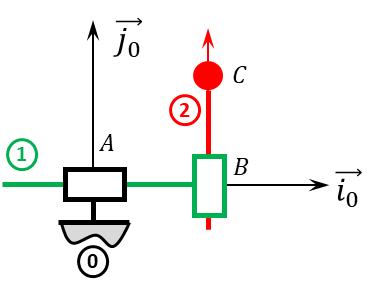
\includegraphics[width=.6\linewidth]{03_TT_01}
\end{center}
\fi

\question{Tracer le graphe des liaisons.}
\ifprof
\else
\fi

\question{Retracer le schéma cinématique pour $\lambda=\SI{10}{mm}$ et $\mu=\SI{10}{mm}$.}
\ifprof
\else
\fi

\question{Retracer le schéma cinématique pour $\lambda=\SI{0}{mm}$ et $\mu=\SI{20}{mm}$.}
\ifprof
\else
\fi


\ifprof
\else
\begin{flushright}
\footnotesize{Corrigé  voir \ref{B2:12:03}.}
\end{flushright}%
\fi


